\begin{figure}
  \centering
  \begin{subfigure}[b]{0.35\textwidth}
    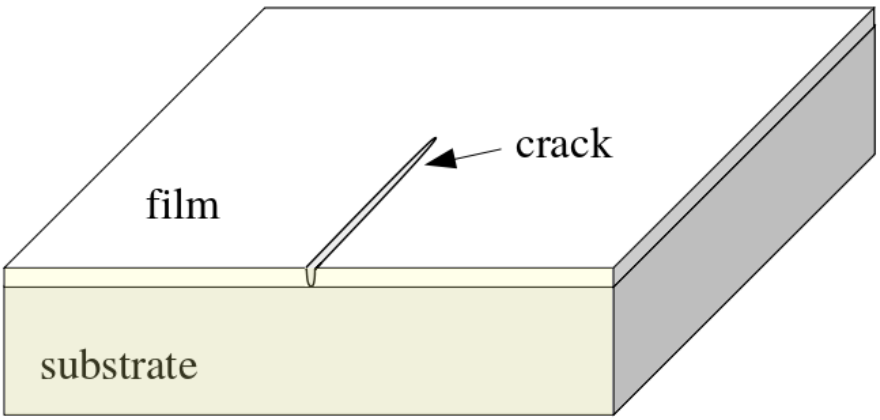
\includegraphics[width=\textwidth,scale=0.5]{Chapter4/figures/1D/side_view.png}
    \caption{}
  \end{subfigure}
  \begin{subfigure}[b]{0.45\textwidth}
    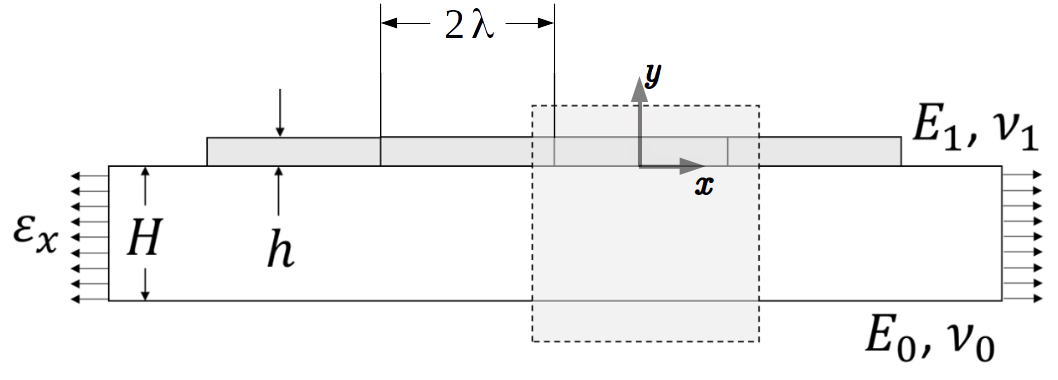
\includegraphics[width=\textwidth,scale=0.5]{Chapter4/figures/1D/1D_schematic.png}
    \caption{}
    \label{fig: Chapter4/1D/schematic}
  \end{subfigure}
  \caption[Description of a one-dimensional model for thin-film cracking.]{Description of a one-dimensional model for thin-film cracking.  (a) Side view  (highlighted in yellow) of the geometry (b) schematic representation of the side view. The elasticity solution is derived for the region highlighted with the shaded box, i.e.\ between the two discontinuities across the thin film. The coordinate system is centered at the middle of the bottom surface of the thin film. }
  \label{fig: Chapter4/1D/simplification}
\end{figure}
